\documentclass[final, usenames, dvipsnames]{beamer}

\title{Real Time Shape Reconstruction for Near Earth Asteroid Landing}
\author{Shankar kulumani}
\year=2018
\subtitle{\the\year~SEAS Student Research and Development Showcase}
\institute{Flight Dynamics and Controls Laboratory (Dr. Taeyoung Lee)\\Department of Mechanical and Aerospace Engineering, School of Engineering and Applied Science}

\mode<presentation>{\usetheme{GWU}}
\usepackage{poster_packages}
\input{my_macros}
\usepackage[orientation=landscape,size=custom,scale=1.32, width=121.92, height=91.44]{beamerposter} 
% \beamertemplategridbackground[0.1cm] % grid for aligning stuff

%\setlength{\abovecaptionskip}{0.1cm}
%\setlength{\belowcaptionskip}{-0.3cm}

\def\newblock{} % Avoid the "\newblock undefined" error. See http://newsgroups.derkeiler.com/Archive/Comp/comp.text.tex/2008-07/msg00381.html"

%-----------------------------------------------------------
\newlength{\colsep}
\newlength{\onecolwidth}
\newlength{\twocolwidth}
\newlength{\figheight}
\setlength{\figheight}{0.15\textheight}
%\setlength{\onecolwidth}{0.23\textwidth} % Width of one column
%\setlength{\twocolwidth}{0.49\textwidth} % Width of two columns
\setlength{\onecolwidth}{28cm} % Width of one column
\setlength{\twocolwidth}{59cm} % Width of two columns
\newlength{\columnheight}
\setlength{\columnheight}{76.5cm}

\setbeamersize{text margin left=1.0cm,text margin right=1.0cm}

\listfiles

%-----------------------------
% MACROS
%-----------------------------
\def\Emph{\textcolor{RoyalBlue}}

%----------------------------------------------------------------------------------------

\begin{document}
\begin{frame}[t] % enclose entire poster in a frame
\begin{columns}[T,onlytextwidth] % start of all columns in poster

%-----------------------------------------------------------------------------------------
% FIRST (LEFT) COLUMN
%---------------------------------------------------------------------------------------
    \begin{column}{\onecolwidth} % first column start

        \begin{block}{Introduction} % Background block
            \begin{itemize}
                \item Asteroids and comets are of significant interest 
                    \begin{itemize}
                        \item \Emph{Science} - Insight into early solar system formation
                        \item \Emph{Mining} - vast quantities of useful materials
                        \item \Emph{Impact} - high risk from hazardous Near-Earth asteroids
                    \end{itemize}
                \item Near-Earth asteroids (NEAs) are especially interesting 
                    \begin{itemize}
                        \item Orbit close to the Earth and are easily accessible
                        \item Many asteroids hold vast quantities of useful materials
                        \item Asteroid mining: Precious metals, propulsion fuels, semiconductors
                        \item Commercialization is feasible with huge amounts of possible profit 
                    \end{itemize}
                \item High probability of future asteroid impacts
            \end{itemize}
            \vspace{0.2in}
            \begin{figure}
                \centering
                \subcaptionbox{Asteroid Mining\label{fig:ast_mining}}{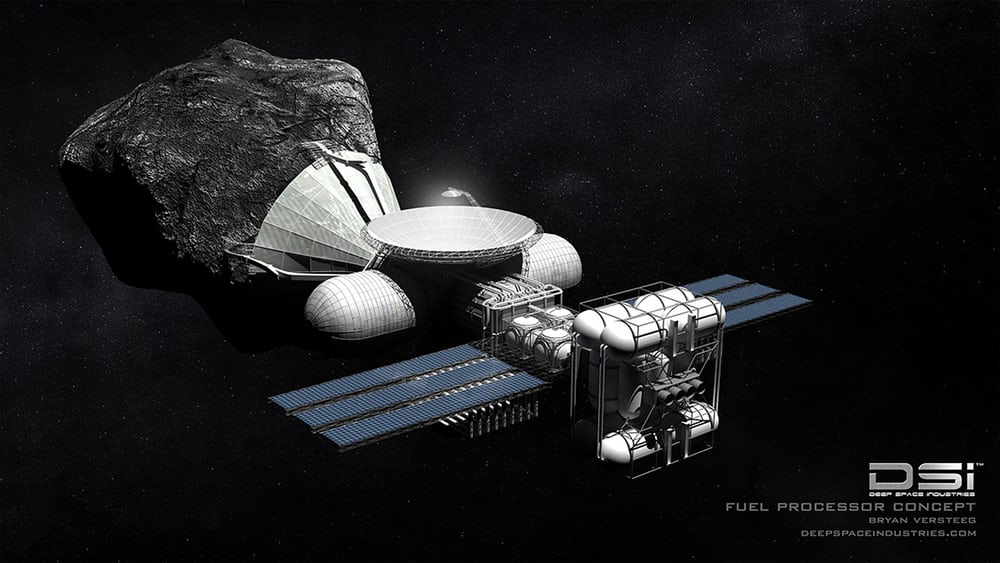
\includegraphics[width=0.4\columnwidth,height=7.3cm]{figures/asteroid-mining-feature-8.jpg}}~
                \subcaptionbox{Asteroid Impact\label{fig:ast_impact}}{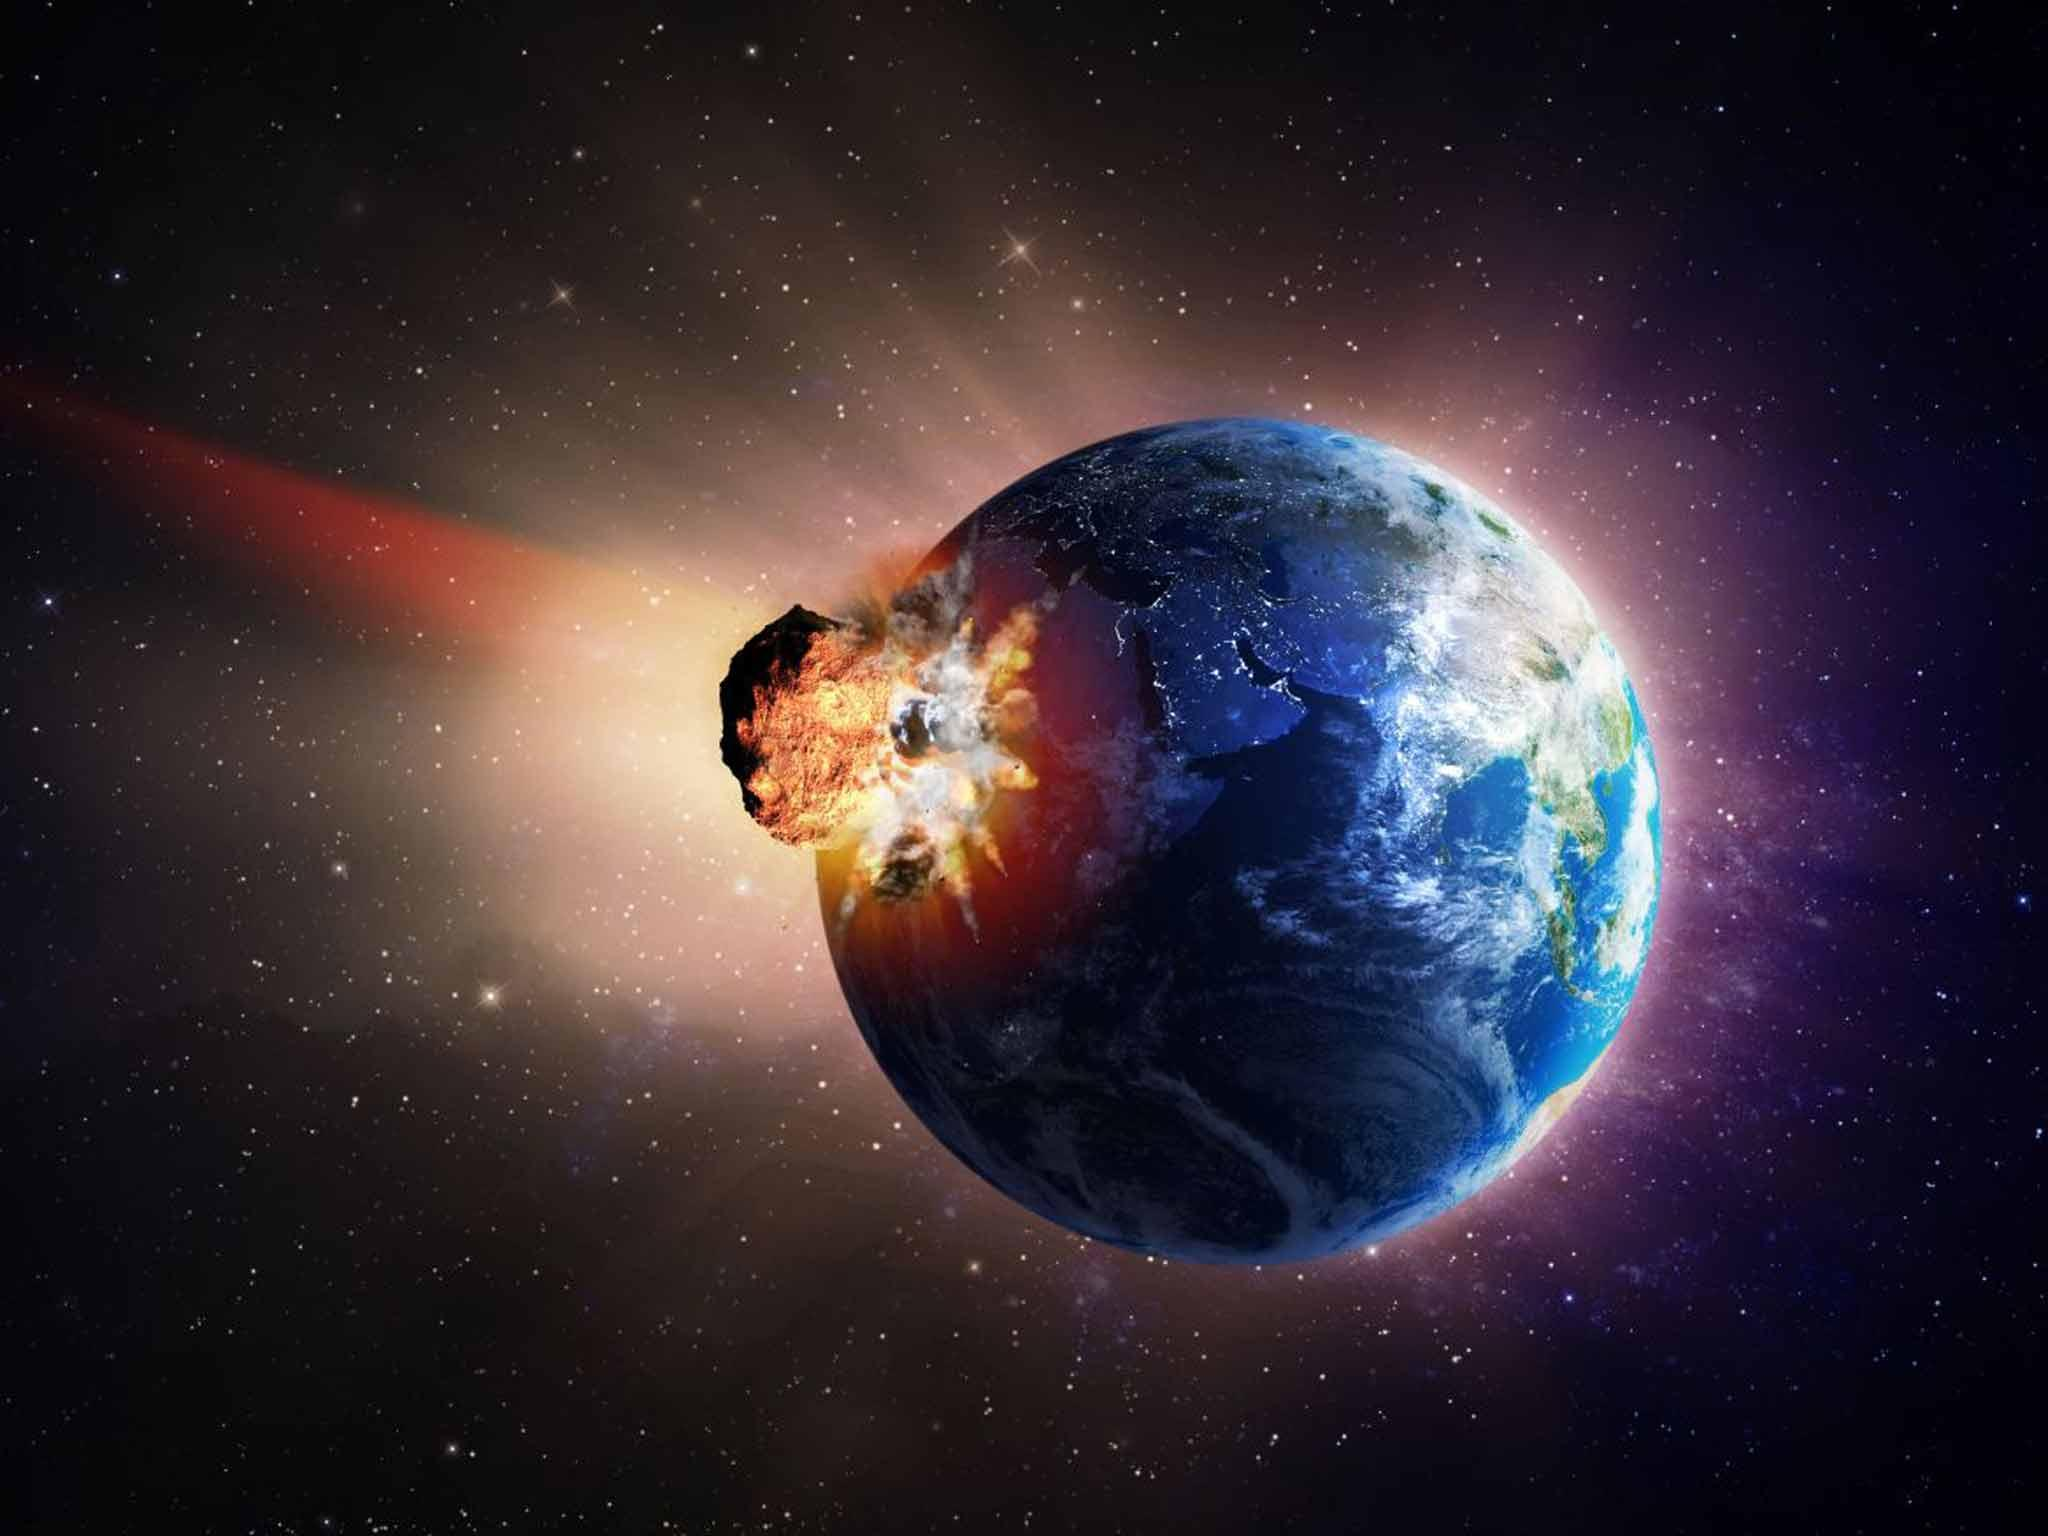
\includegraphics[width=0.4\textwidth,height=7.3cm,keepaspectratio]{figures/asteroid-alamy.jpg}}
            \end{figure}
            \vspace*{0.2cm}
        \end{block} % end of background block

        \begin{block}{Technical Challenges}
            \begin{itemize}
                \item Unknown asteroid shape and dynamics
                    \begin{itemize}
                        \item Only a rough estimate of the shape and mass of asteroid is possible from Earth
                        \item At arrival, spacecraft is flying into an unknown environment 
                        \item Spacecraft must autonomously survey the asteroid and handle unknown perturbations
                    \end{itemize}
                \item Astrodynamic trajectory design is complicated
                    \begin{itemize}
                        \item Highly nonlinear and chaotic dynamics requires intuition by designer
                        \item Using low-thrust propulsion adds additional difficulties in accurately capturing the small perturbations
                    \end{itemize}
                \item Difficult to find 3D asteroid shape from the Earth
                    \begin{itemize}
                        \item Current method requires extensive mapping period
                        \item Exact shape is critical for close-proximity missions - shape defines the gravity
                        \item Improve the state of the art to allow for missions without prior shape knowledge
                    \end{itemize}
            \end{itemize}
            \vspace*{0.2cm}
        \end{block} 

        \begin{block}{Shape/Gravitational Modeling}
            \begin{itemize}
                \item Asteroids are extended bodies - not point masses
                    \begin{itemize}
                        \item Gravity is the key force in orbital mechanics
                        \item An accurate representation of gravity is critical to accurate and realistic analysis
                    \end{itemize}
                \item \Emph{Polyhedron Gravitational model} used to represent the asteroid
                    \begin{itemize}
                        \item Globally valid and closed-form analytical solution for gravity
                        \item Exact potential assumes a constant density assumption
                        \item Accuracy is only dependent on the shape
                    \end{itemize}
                    \[
                        U(\vecbf{r}) = \frac{1}{2} G \sigma \sum_{e \in
                        \text{edges}} \vecbf{r}_e \cdot \vecbf{E}_e \cdot
                        \vecbf{r}_e \cdot L_e - \frac{1}{2}G \sigma \sum_{f \in
                        \text{faces}} \vecbf{r}_f \cdot \vecbf{F}_f \cdot
                        \vecbf{r}_f \cdot \omega_f 
                    \]	
                \item Gravity defined solely as a function of shape
                    \begin{itemize}
                        \item Autonomous and agile reconstruction of shape from spacecraft measurements is required
                        \item Avoid long delays/costs with ground based processing
                        \item Enable quick response landing or operations near asteroid 
                        \item Allow for a much wider class of potential missions and operations
                    \end{itemize}
            \end{itemize}
            \vspace*{0.25cm}
        \end{block} 
\end{column}  % first column end

%-----------------------------------------------------------------------------------------
% SECOND (WIDE MIDDLE) COLUMN
%---------------------------------------------------------------------------------------
\begin{column}{\twocolwidth}
\begin{block}{Controlled Dynamics around NEAR Earth Asteroids} % structure block
	\begin{minipage}{0.5\columnwidth} % left half of this block
	\begin{itemize}
            \item Spacecraft is modeled as a rigid dumbbell
                \begin{itemize}
                    \item Simple model of two masses connected by a massless rod 
                        \begin{figure}
                            \centering
                            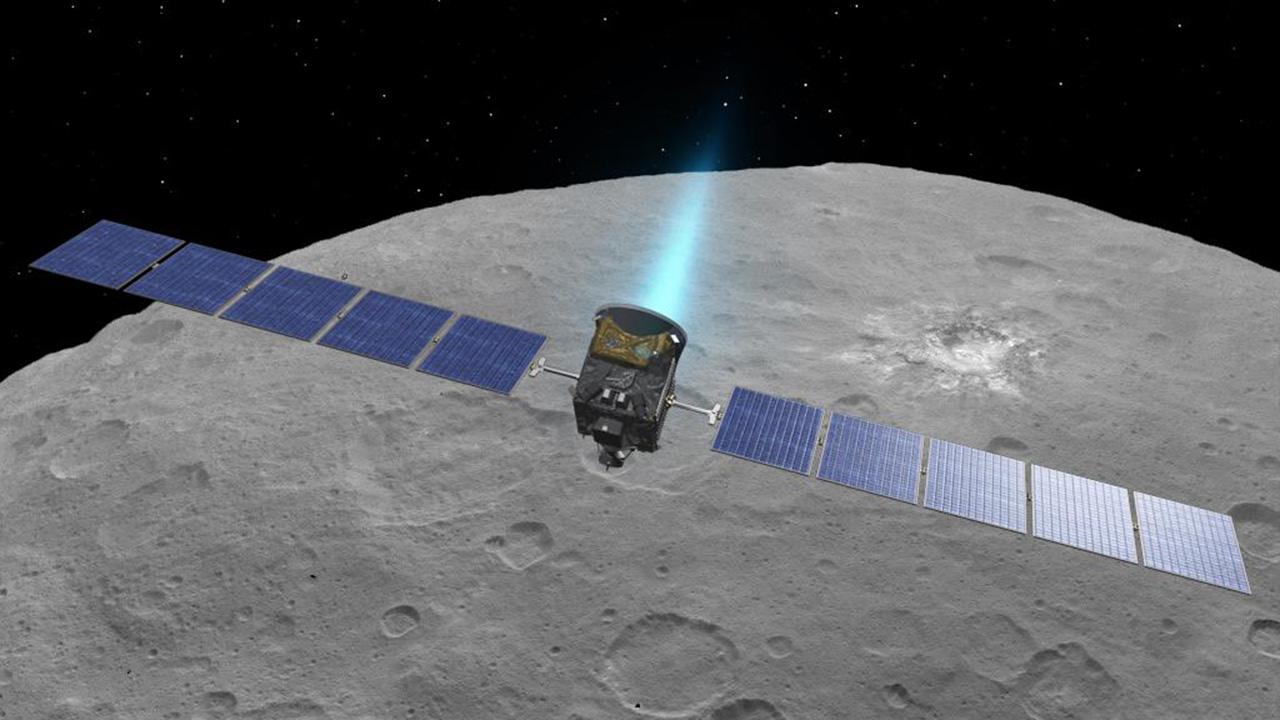
\includegraphics[width=0.6\columnwidth]{figures/dawn.jpg}
                        \end{figure}
                    \item Accurately captures the complex interaction of rotation and gravititational gradient
                \end{itemize}
            \item Translational and Rotational Motion is tightly coupled
                \begin{align*}
                    \dot{\vb{x}} &= \vb{v}, \\
                    \parenth{m_1 + m_2} \dot{\vecbf{v}} &= m_1 R_A \deriv{U}{\vecbf{z}_1} + m_2 R_A \deriv{U}{\vecbf{z}_2} + \vecbf{u}_f, \\
                    \dot{R} &= R S(\vb{\Omega}) , \\
                    J \dot{\vecbf{\Omega}} + \vecbf{\Omega} \times J \vecbf{\Omega} &= \vecbf{M}_1 + \vecbf{M}_2 + \vecbf{u}_m. 
                \end{align*}

	\end{itemize}
	\end{minipage}% end of left half of block
	\begin{minipage}{0.5\columnwidth}% right half of block
        \begin{itemize}
            \item Spacecraft is operating around \Emph{Itokawa} and \Emph{Castalia}
            \begin{itemize}
                \item Potentially hazardous near Earth asteroids which cross our orbit 
                \item 25413 Itokawa, discovered in 1998, with axes \( 535 \times 294 \times 209 \si{\meter}\)
                \item 4769 Castalia, discovered in 1989, with axes \( 1800 \times 800 \times 800 \si{\meter}\) 
                \item Truth shape models generated using previous spacecraft missions
            \end{itemize}
        \end{itemize}
        \begin{figure}
            \centering
            % \subcaptionbox{25413 Itokawa\label{fig:itokawa}}{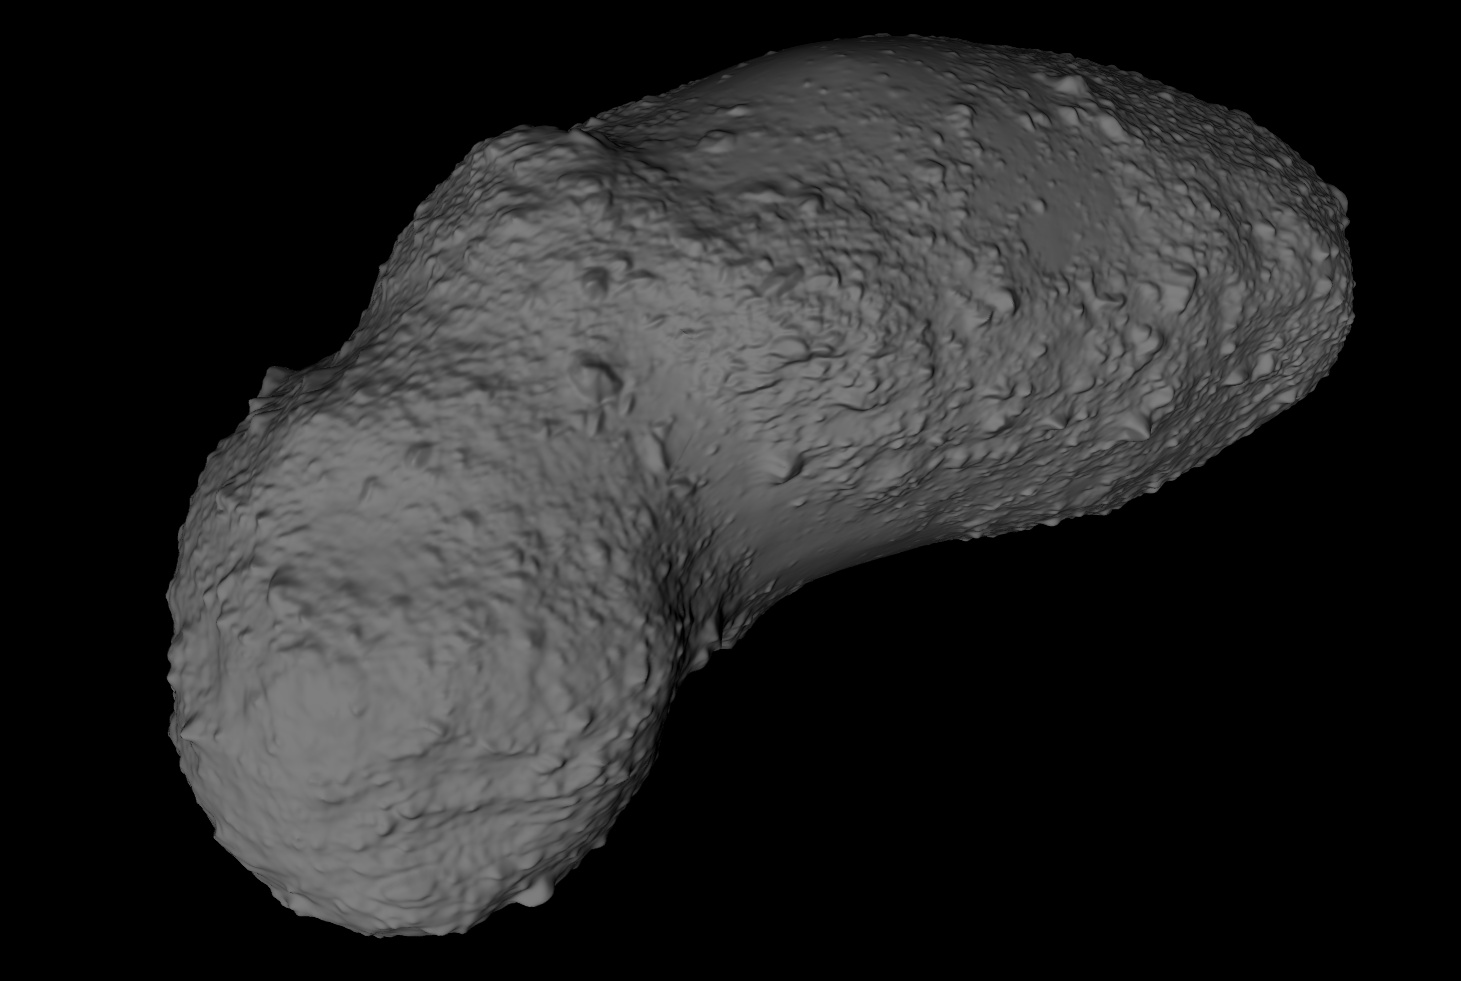
\includegraphics[width=0.4\columnwidth,height=0.15\columnheight]{figures/itokawa.jpg}}~
            \subcaptionbox{4769 Castalia\label{fig:castalia}}{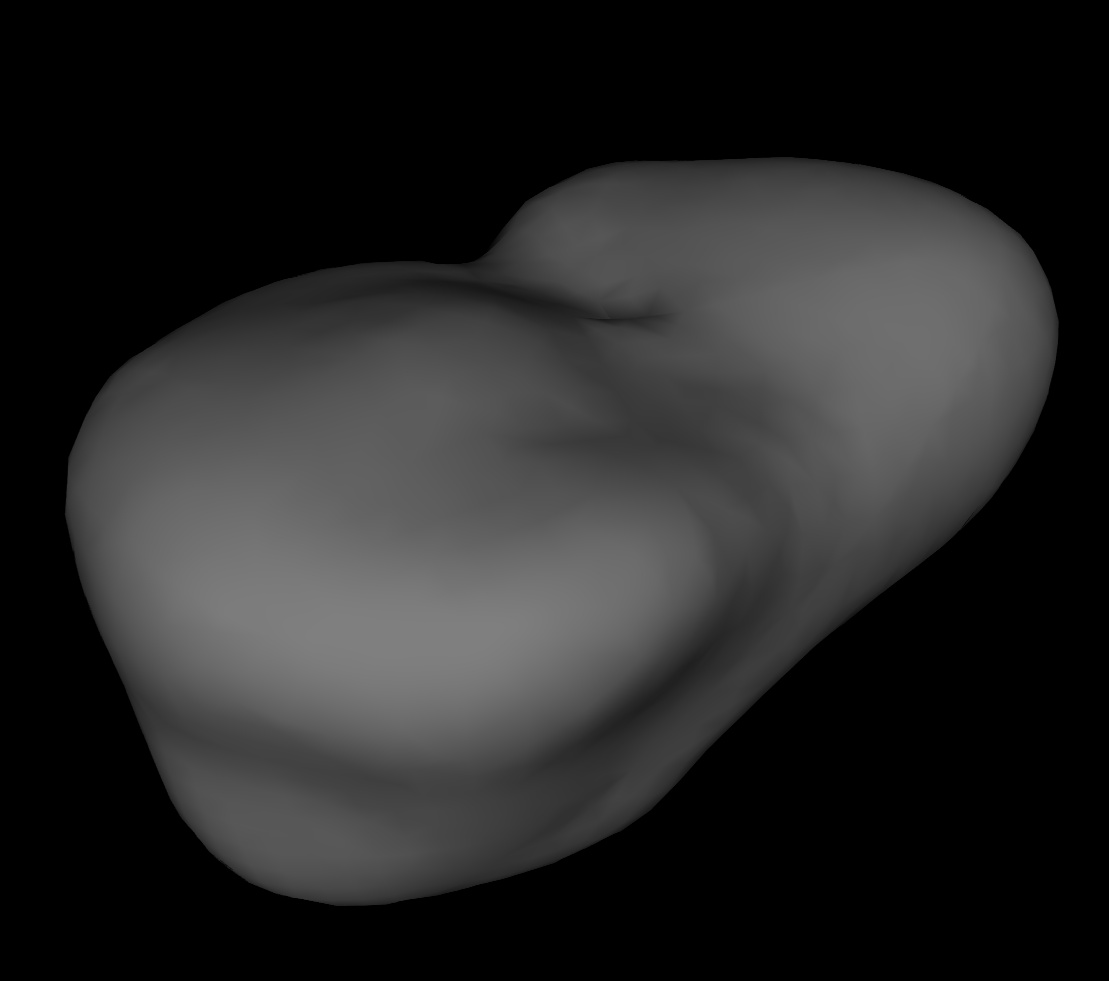
\includegraphics[keepaspectratio,width=0.7\columnwidth]{figures/castalia.jpg}}
        \end{figure}
	\end{minipage}%end of right half of block
\end{block} % end of structure block

\begin{block}{Shape model reconstruction from LIDAR} % results block
    \begin{minipage}[t]{0.5\columnwidth}
    \begin{itemize}
        \item Reconstruct the shape of Itokawa from LIDAR
            \begin{itemize}
                \item Powerful laser is used to accurately measure the distance from spacecraft to surface of asteroid
                \item Accurate timing used to measure the total time of flight \( d = c \frac{t}{2} \)
            \end{itemize}
        \item Multiple scans of the surface creates a point cloud representation of asteroid
        \begin{itemize}
            \item Immense collection of points capture the surface topology
            \item Surface reconstruction is used to transform the cloud into a mesh 
            \item Mesh representation is required for polyhedron potential model
        \end{itemize}
    \end{itemize}
    \end{minipage}~
    \begin{minipage}[t]{0.48\columnwidth}
    \begin{itemize}
        \item Spacecraft with LIDAR around two Near Earth asteroids
            \begin{itemize}
                \item Only Itokawa was visited by a real spacecraft - much higher resolution data is available
            \end{itemize}
        \item Spacecraft inertially ``hovering'' while asteorid rotates 
            \begin{itemize}
                \item Coupled motion of spacecraft is controlled 
                \item Inertially Fixed and pointed at asteroid
            \end{itemize}
        \item LIDAR measurements occur at \SI{1}{\hertz} 
        \item \Emph{Point Cloud} used to reconstruct the mesh
    \end{itemize}
    \end{minipage}
    \vspace{1cm}
    \begin{figure}
        \centering
        \subcaptionbox{Itokawa LIDAR\label{fig:itokawa_lidar}}{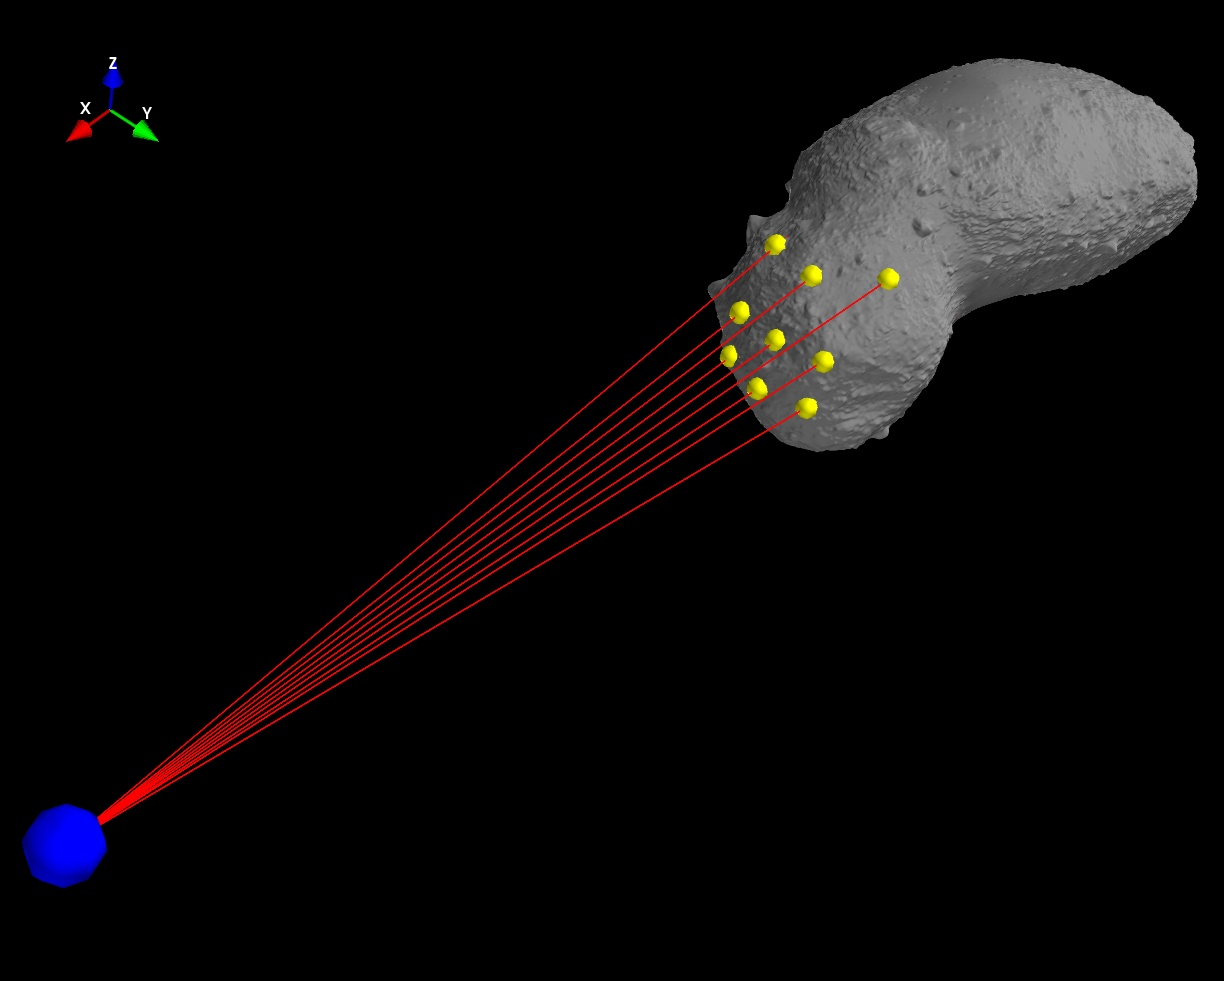
\includegraphics[width=0.3\textwidth,height=\figheight]{figures/itokawa_lidar.jpg}}~
        \subcaptionbox{Itokawa Point Cloud\label{fig:itokawa_point_cloud}}{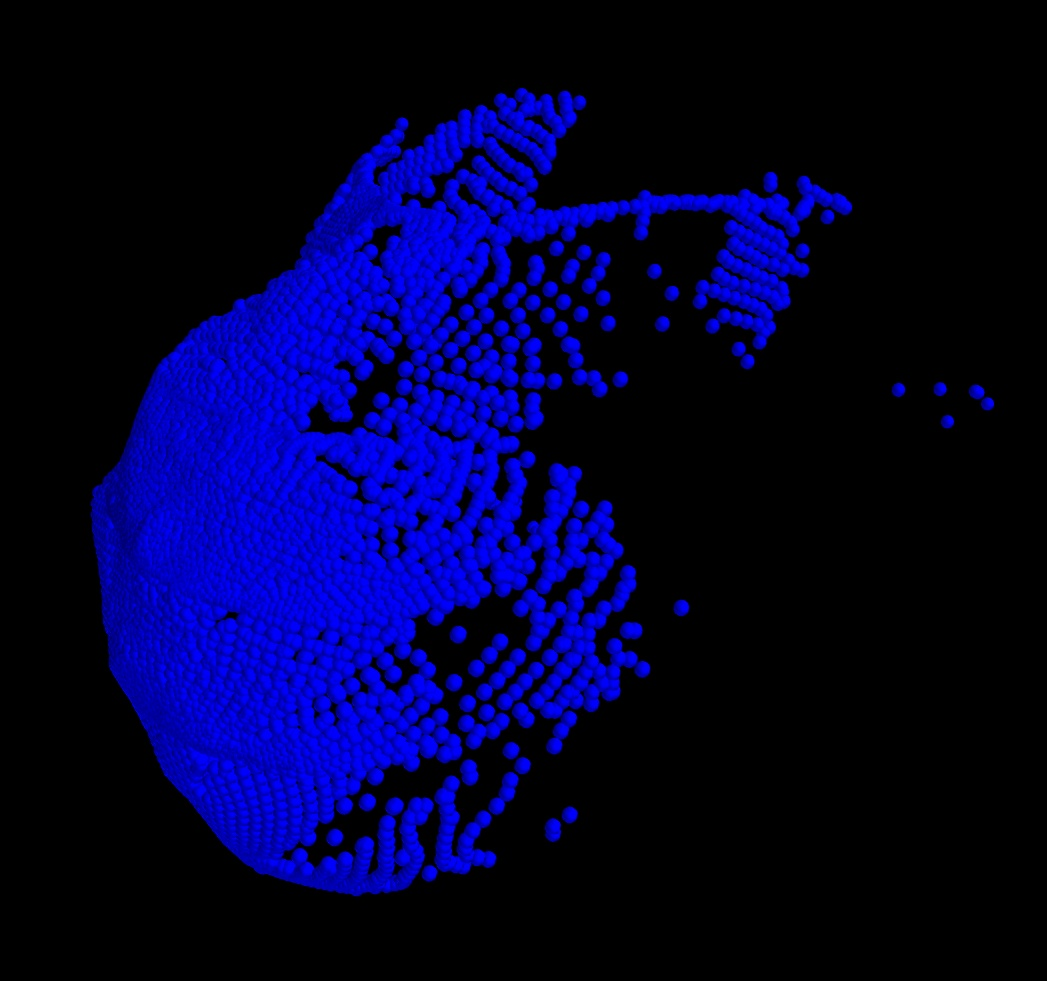
\includegraphics[width=0.3\textwidth,height=\figheight]{figures/itokawa_point_cloud}}~
        \subcaptionbox{Itokawa Mesh\label{fig:itokawa_mesh}}{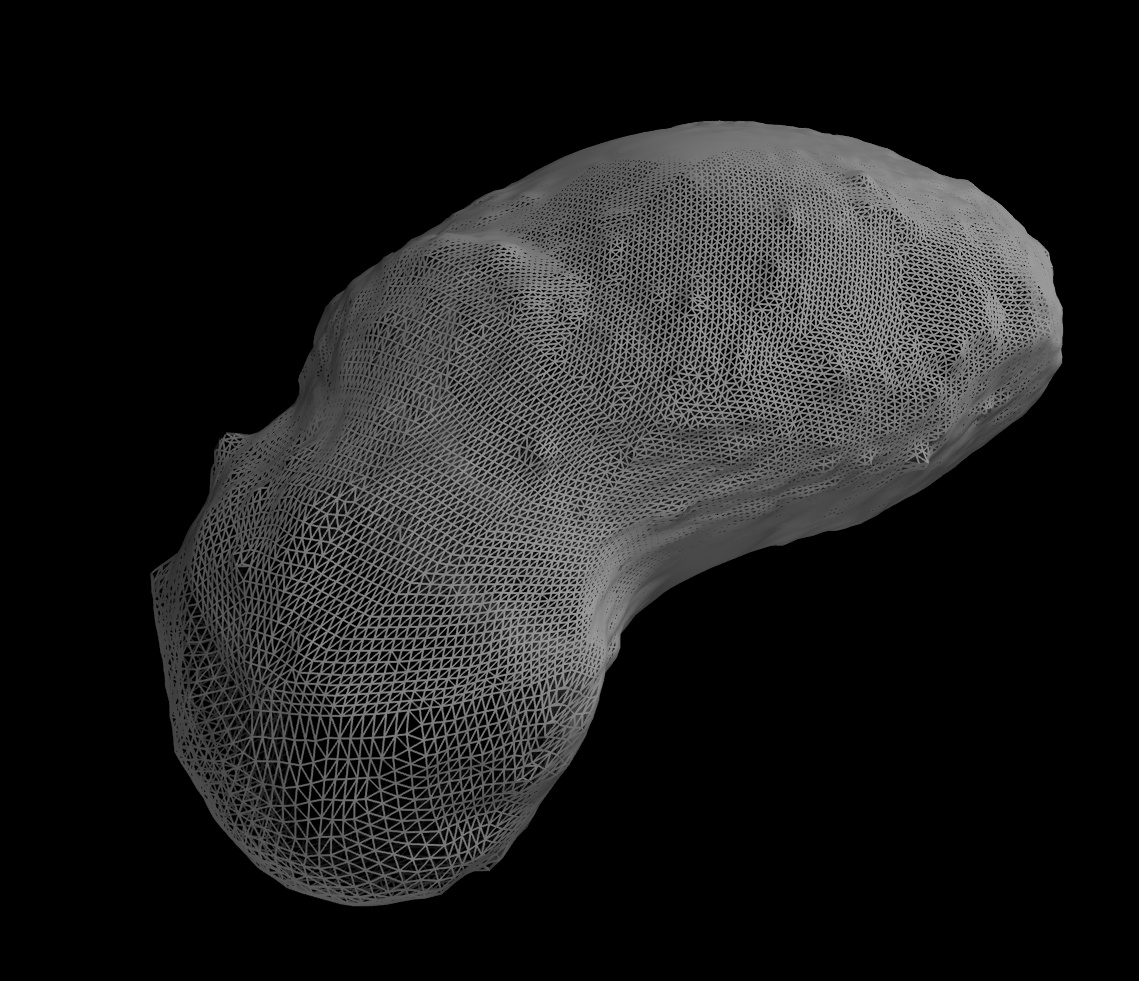
\includegraphics[width=0.3\textwidth,height=\figheight]{figures/itokawa_wireframe.jpg}}\\

        \subcaptionbox{Castalia LIDAR\label{fig:castalia_lidar}}{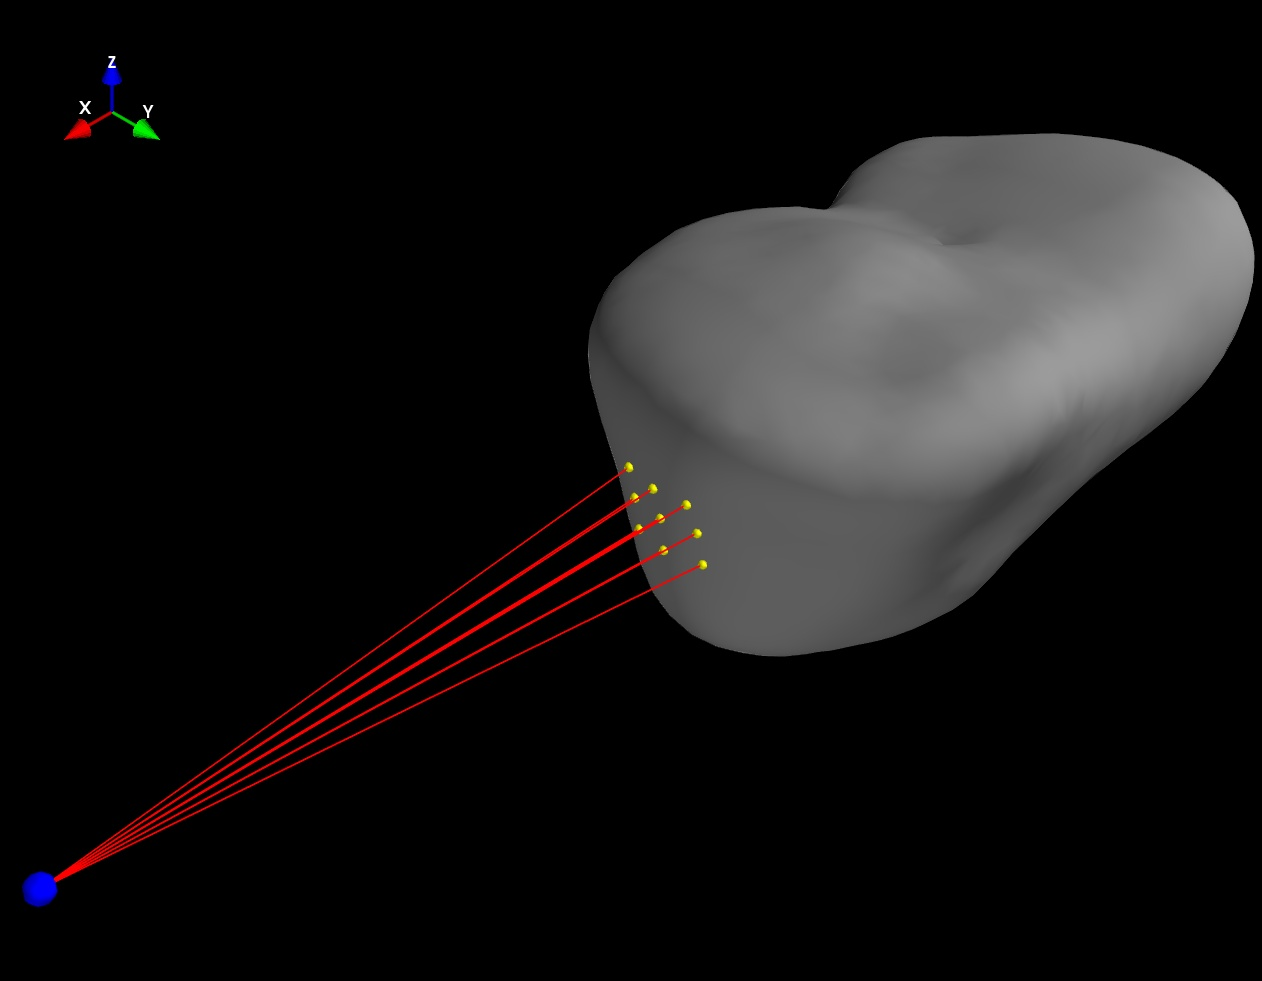
\includegraphics[width=0.3\textwidth,height=\figheight]{figures/castalia_lidar.jpg}}~
        \subcaptionbox{Castalia Point Cloud\label{fig:castalia_point_cloud}}{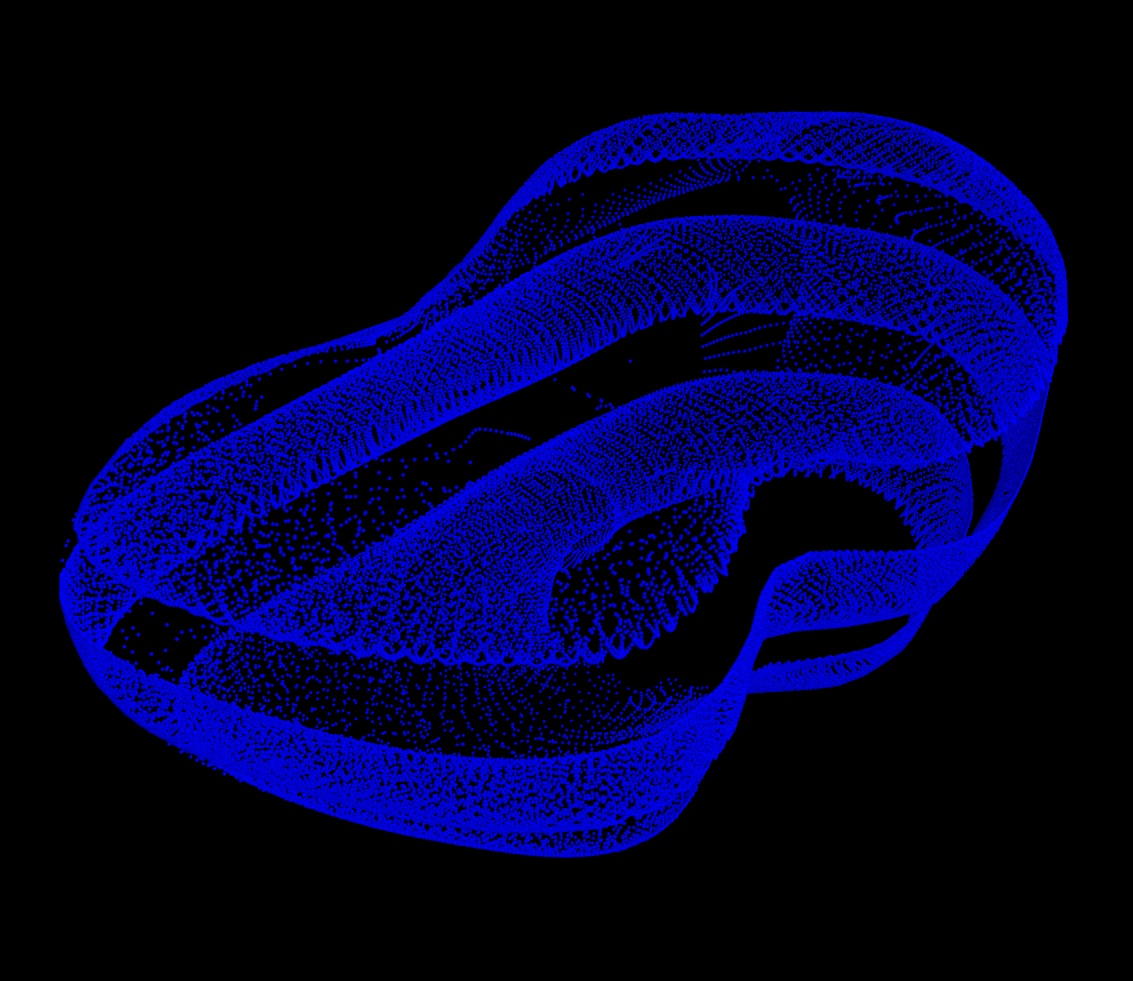
\includegraphics[width=0.3\textwidth,height=\figheight]{figures/castalia_point_cloud.jpg}}~
        \subcaptionbox{Castalia Mesh\label{fig:castalia_mesh}}{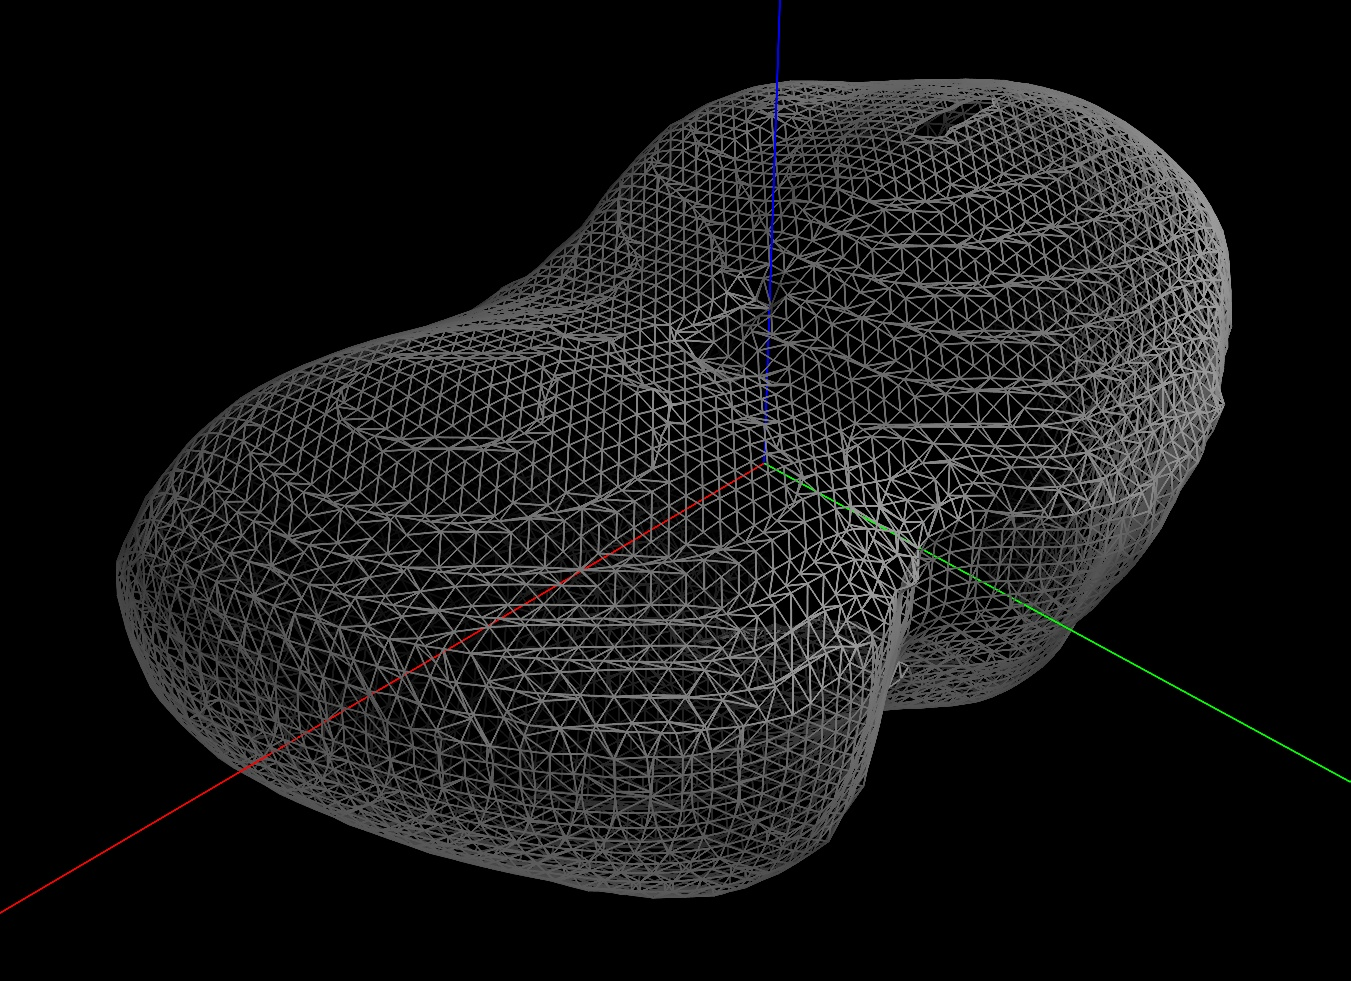
\includegraphics[width=0.3\textwidth,height=\figheight]{figures/castalia_wireframe.jpg}}
    \end{figure}
    \vspace*{0.1cm}
\end{block} % end of results block
\end{column}


%-----------------------------------------------------------------------------------------
% THIRD (RIGHT) COLUMN
%---------------------------------------------------------------------------------------
\begin{column}{\onecolwidth} % third column start

\begin{block}{Computational Geometry}
    \begin{itemize}
        \item \Emph{Computational Geometry} is the study of algorithms and data structures for operating on geometric objects
            \begin{itemize}
                \item Extensive use in a variety of fields such as computer graphics, robotics, and mechanical design
            \end{itemize}
        \item Asteroid shape is defined as a \Emph{polyhedron}
        \begin{itemize}
            \item 3D generalization of a polygon into a mesh
            \item Shape is defined from a list of vertices and connections between vertices to form triangular faces
        \end{itemize}
    \item Geometric algorithms and tools use to efficiently operate on the points to form a mesh
        \begin{itemize}
            \item Determine intersection of a ray and the surface
            \item Determine closest point to a mesh
            \item Integrate a new vertex into a mesh
        \end{itemize}
    \item Efficient computational algorithms and data structures allows for improvements over current methods
        \begin{enumerate}
            \item Generate LIDAR measurement
            \item Find closest point on mesh
            \item Incorporate measurement as new vertex in mesh
            \item Rebuild mesh and triangulation
        \end{enumerate}
    \end{itemize}

    \begin{figure}
        \centering
        \subcaptionbox{Vertex\label{fig:vertex}}{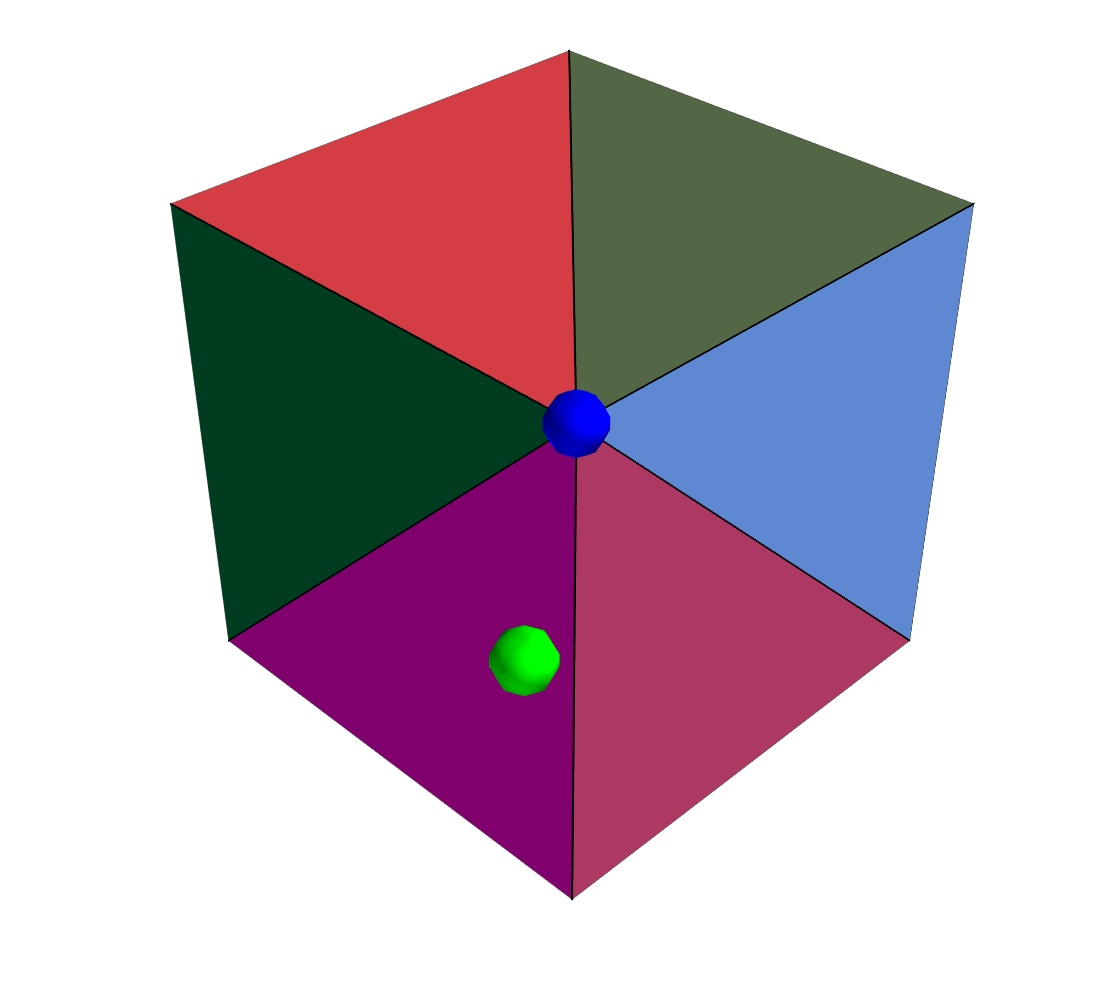
\includegraphics[width=0.465\textwidth,clip,trim={4cm 0 4cm 0}]{figures/cube_vertex.jpg}}~   
        \subcaptionbox{Edge\label{fig:edge}}{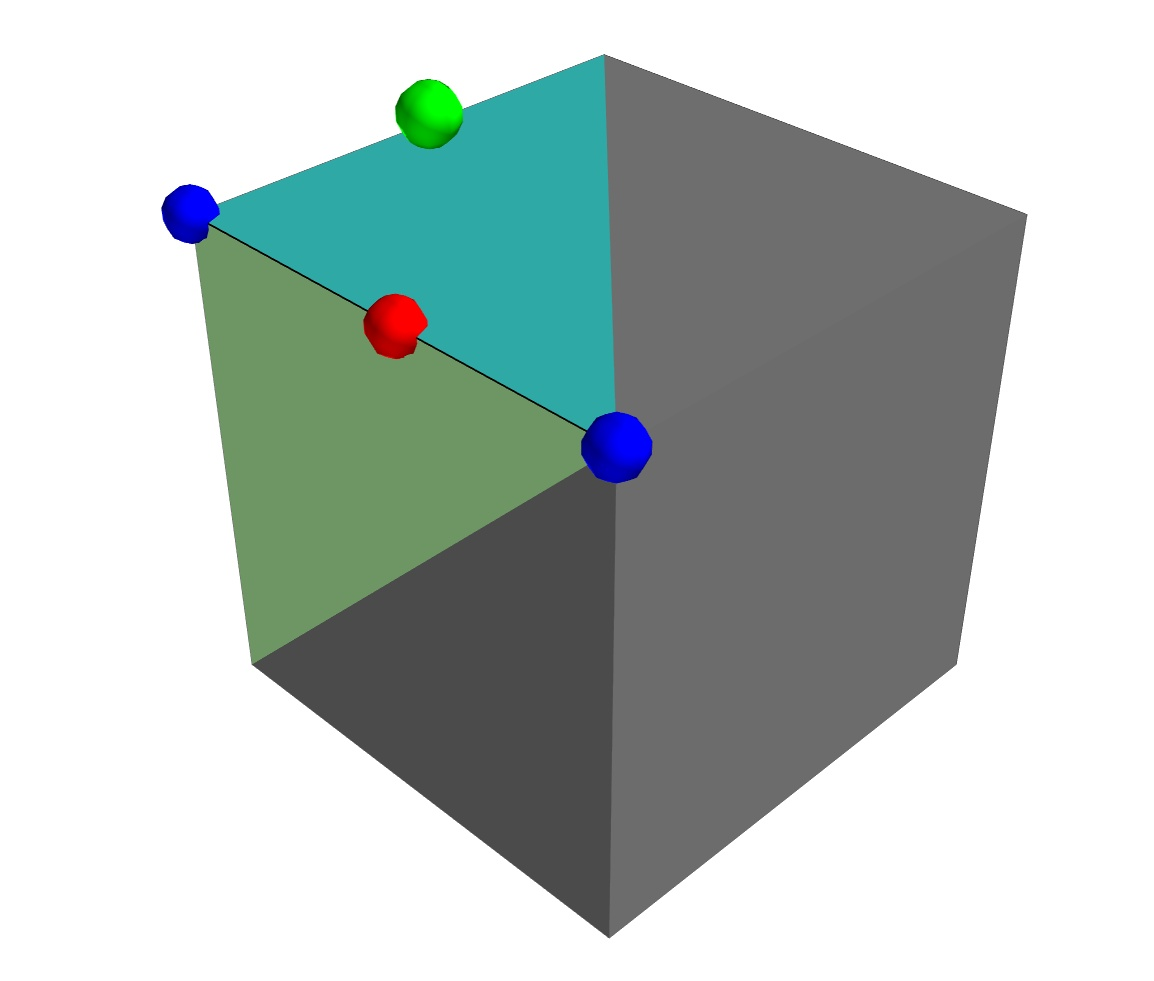
\includegraphics[width=0.465\textwidth,clip,trim={4cm 0 4cm 0}]{figures/cube_edge.jpg}}\\

        \subcaptionbox{Face\label{fig:face}}{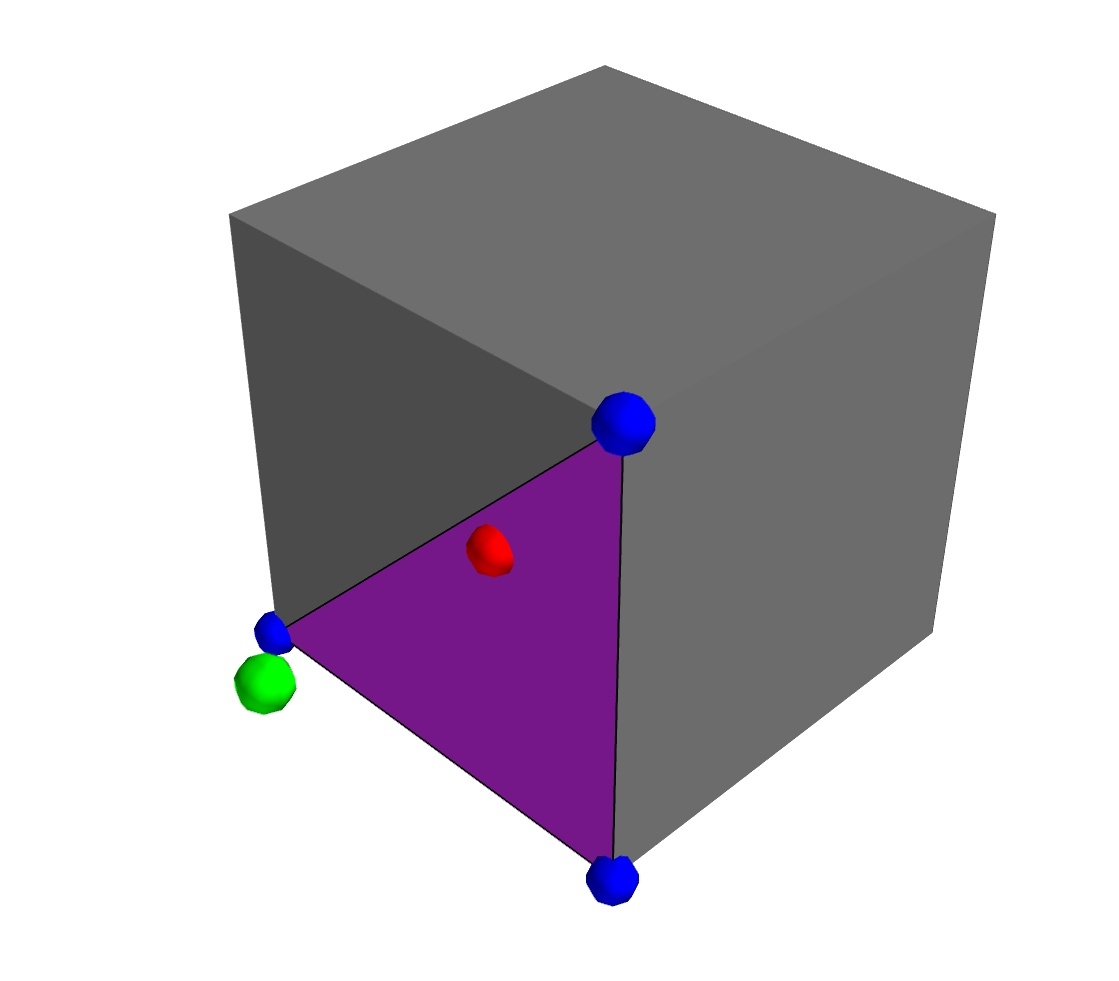
\includegraphics[width=0.465\textwidth,clip,trim={4cm 0 4cm 0}]{figures/cube_face.jpg}}
    \end{figure}
\end{block}

\begin{block}{Conclusions} % conclusion
    \begin{itemize}
        \item Shape reconstruction of an asteroid from LIDAR measurements
            \begin{itemize}
                \item Reduce the amount of time required for mapping of the asteroid
                \item Incrementaly build shape of asteroid in real time
                \item Enables updated dynamic model for control system
                \item Allows for complex close-proximity missions without the need for long duration mapping period
            \end{itemize}
        \item Future work will incorporate further enhancements
            \begin{itemize}
                \item Complex dynamics requires accurate integration schemes - \Emph{Variational Integrators}
                \item Utilize sensor measurements to estimate spacecraft and asteroid state estimation
            \end{itemize}
    \end{itemize}
\end{block} % conclusion
\end{column}  % third column end

\end{columns} % end of all columns in poster
\end{frame} % end of enclosing frame
\end{document}
